% DO NOT COMPILE THIS FILE DIRECTLY!
% This is included by the other .tex files.

\begin{frame}[t,plain]
\titlepage
\end{frame}

\section{Introduction}
\begin{frame}
    \frametitle{\texttt{\$whoarewe} - MISP and CIRCL}
    \begin{center}
        
\includegraphics[width=1.0\textwidth]{misp-banner.png}
    \end{center}
    \begin{center}
        
\includegraphics[width=0.35\textwidth]{circl.png}
    \end{center}
    \begin{itemize}
        \item CIRCL is mandated by the Ministry of the Economy (under NIS 2).
        \item CIRCL leads the development of MISP.
        \item {\bf CIRCL manages multiple large MISP communities, enabling active daily threat intelligence sharing.}
        \item Funding comes from Luxembourg, various EU programs, and partnerships under EU/US agreements.
    \end{itemize}
\end{frame}

\begin{frame}
    \frametitle{Plan of this Session}
    \begin{itemize}
        \item MISP Intro: What it is, and what it can do
        \item Data Distribution and Sharing models
        \item Demo: Correlation with traditional Cybercrime
        \item Demo: Election Security
    \end{itemize}
\end{frame}

\begin{frame}
    \frametitle{What is MISP?}
    \begin{itemize}
        \item MISP\footnote{\url{https://www.misp-project.org/}} is a {\bf threat intelligence sharing platform} ({\bf TISP}) that is \underline{FREE} \& \underline{OPEN SOURCE} software
        \item Mature project that started in 2012, and has been following a community-driven development since then
    \end{itemize}

    \begin{center}
        
\includegraphics[width=0.99\linewidth]{release_overtime.png}
    \end{center}
\end{frame}

\begin{frame}
    \frametitle{What is MISP?}
    \begin{itemize}
        \item Used worldwide to manage and share threat-related information and intelligence.
	\item \textbf{Open-Source Commitment}: Users of MISP can rely on the tool remaining open source and never becoming closed source (autonomy of the users).
    \end{itemize}

    \begin{center}
        
\includegraphics[width=0.99\linewidth]{contributors.png}
    \end{center}
\end{frame}


\begin{frame}
    \frametitle{What is MISP? (1)}
    \begin{itemize}
        \item A tool that {\bf collects} from partners, your analysts, your tools, feeds, $\cdots$
        \item Normalises, {\bf correlates}, {\bf enriches} the data
        \item Allows teams and communities to {\bf collaborate} and {\bf share}
        \item {\bf Feeds} automated protective tools and {\bf disseminate}
    \end{itemize}
\end{frame}

\begin{frame}
    \frametitle{Who is using MISP? (1)}
    \begin{center}
        
\includegraphics[width=0.64\linewidth]{org-count-misppriv.png}
        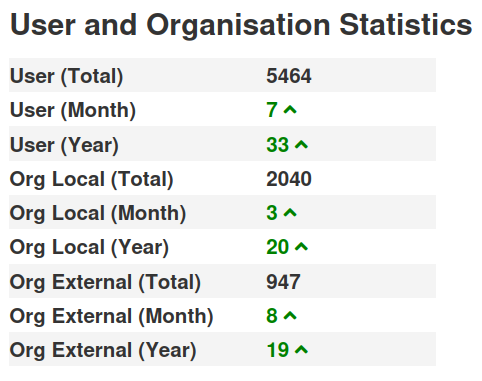
\includegraphics[width=0.35\linewidth]{misppriv-user-stats.png}
    \end{center}
\end{frame}

\begin{frame}
    \frametitle{Who is Using MISP? (2)}
    \textbf{Communities:} Groups of users sharing within a set of common objectives and values.
    \vspace{1em}
    \begin{itemize}
        \item \textbf{Private Sector:} Financial, Manufacturing, Telecommunications.
        \item \textbf{Military and International Organizations:} NATO, military CSIRTs, national and governmental CERTs, etc.
        \item \textbf{Security Vendors:} Running their own communities or interfacing with MISP communities
        \item \textbf{Topical Communities:} Set up to tackle specific issues (e.g., COVID-19 MISP).
        \item \textbf{ISACs:} Serving various sectors such as Telecom, Retail, Aviation Traffic Control, etc.
        \item \textbf{Trusted Groups:} Operating MISP communities in island mode (air-gapped systems) or partially connected modes.
        \item \textbf{Law Enforcement Agencies (LEAs):} EUROPOL, INTERPOL, MISP-LEA, and more.
        \item \textbf{International Groups:} FIRST.org, MISP-Priv, and others.
    \end{itemize}
\end{frame}

\begin{frame}
    \frametitle{What is MISP? (2)}
    MISP is designed from the ground up to perform context-rich \textbf{threat intelligence}:
    \vspace{0.5em}
    \begin{itemize}
           \item {\bf Enrich} information with context and metadata
           \item Maps {\bf Threats and TTPs} (e.g MITRE ATT\&CK)
           \item Supports many {\bf standardized classification} marking
           \item Enables information {\bf curation} through automated quality checks
           \item Offers visualisation of threat {\bf relationships} and \textbf{technique} used
           \item Generates customizable {\bf threat reports}
           \item Allows creation of {\bf Dashboard} for trend analysis
    \end{itemize}
\end{frame}

\begin{frame}
    \frametitle{MISP Project Overview}
    \begin{center}
        
\includegraphics[width=0.85\linewidth]{misp-overview-simplified.pdf}
    \end{center}
\end{frame}


\begin{frame}
    \frametitle{Information Quality Management}
    MISP has many features to help you manage and curate the data:
    \begin{itemize}
        \item \textbf{Correlating} data
        \item Feedback loop from detections via {\bf Sightings}
        \item {\bf False positive management} via the warninglist system
        \item {\bf Enrichment system} via MISP-modules
        \item {\bf Workflow} system to review and control information publication
        \item {\bf Integrations} with a plethora of tools and formats
        \item Flexible {\bf API} and support {\bf libraries} such as PyMISP to ease integration
        \item {\bf Timelines} and giving information a temporal context
        \item Full chain for {\bf indicator life-cycle management}
        \item {\bf Jupyter Notebooks} supporting common use-cases
    \end{itemize}
\end{frame}

\begin{frame}
    \frametitle{Flexible Data Format}
    \begin{center}
        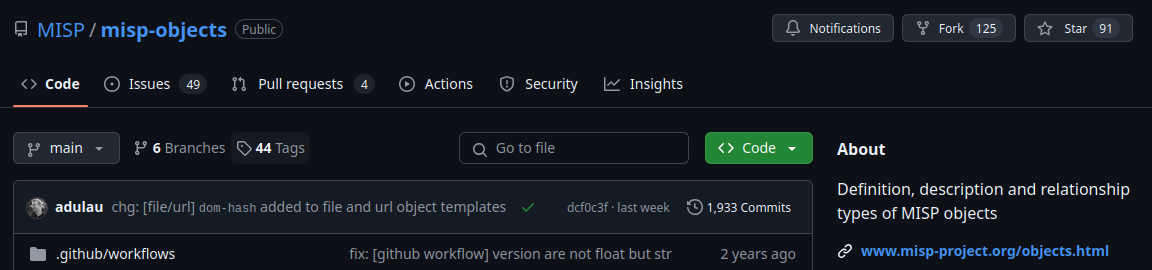
\includegraphics[width=0.84\linewidth]{misp-objects-repo.png}
    \end{center}
    \begin{itemize}
        \item A wide variety of objects template is available and extendable to describe \textbf{any concept}.
        \item Examples:
        \begin{itemize}
            \item \textbf{Network Indicators:} IP addresses, URLs, file hashes, $\cdots$
            \item \textbf{Devices:} Mobile phones, software, other devices.
            \item \textbf{Payment:} Credit cards, transactions, impacts.
            \item \textbf{Vehicles:} Cars, planes.
            \item \textbf{Personal Information:} Passports, persons, identities, PNR.
            \item And \textbf{many more} $\cdots$
        \end{itemize}
    \end{itemize}
\end{frame}

\begin{frame}
    \frametitle{Rich Marking and Knowledge Base}
    \begin{center}
        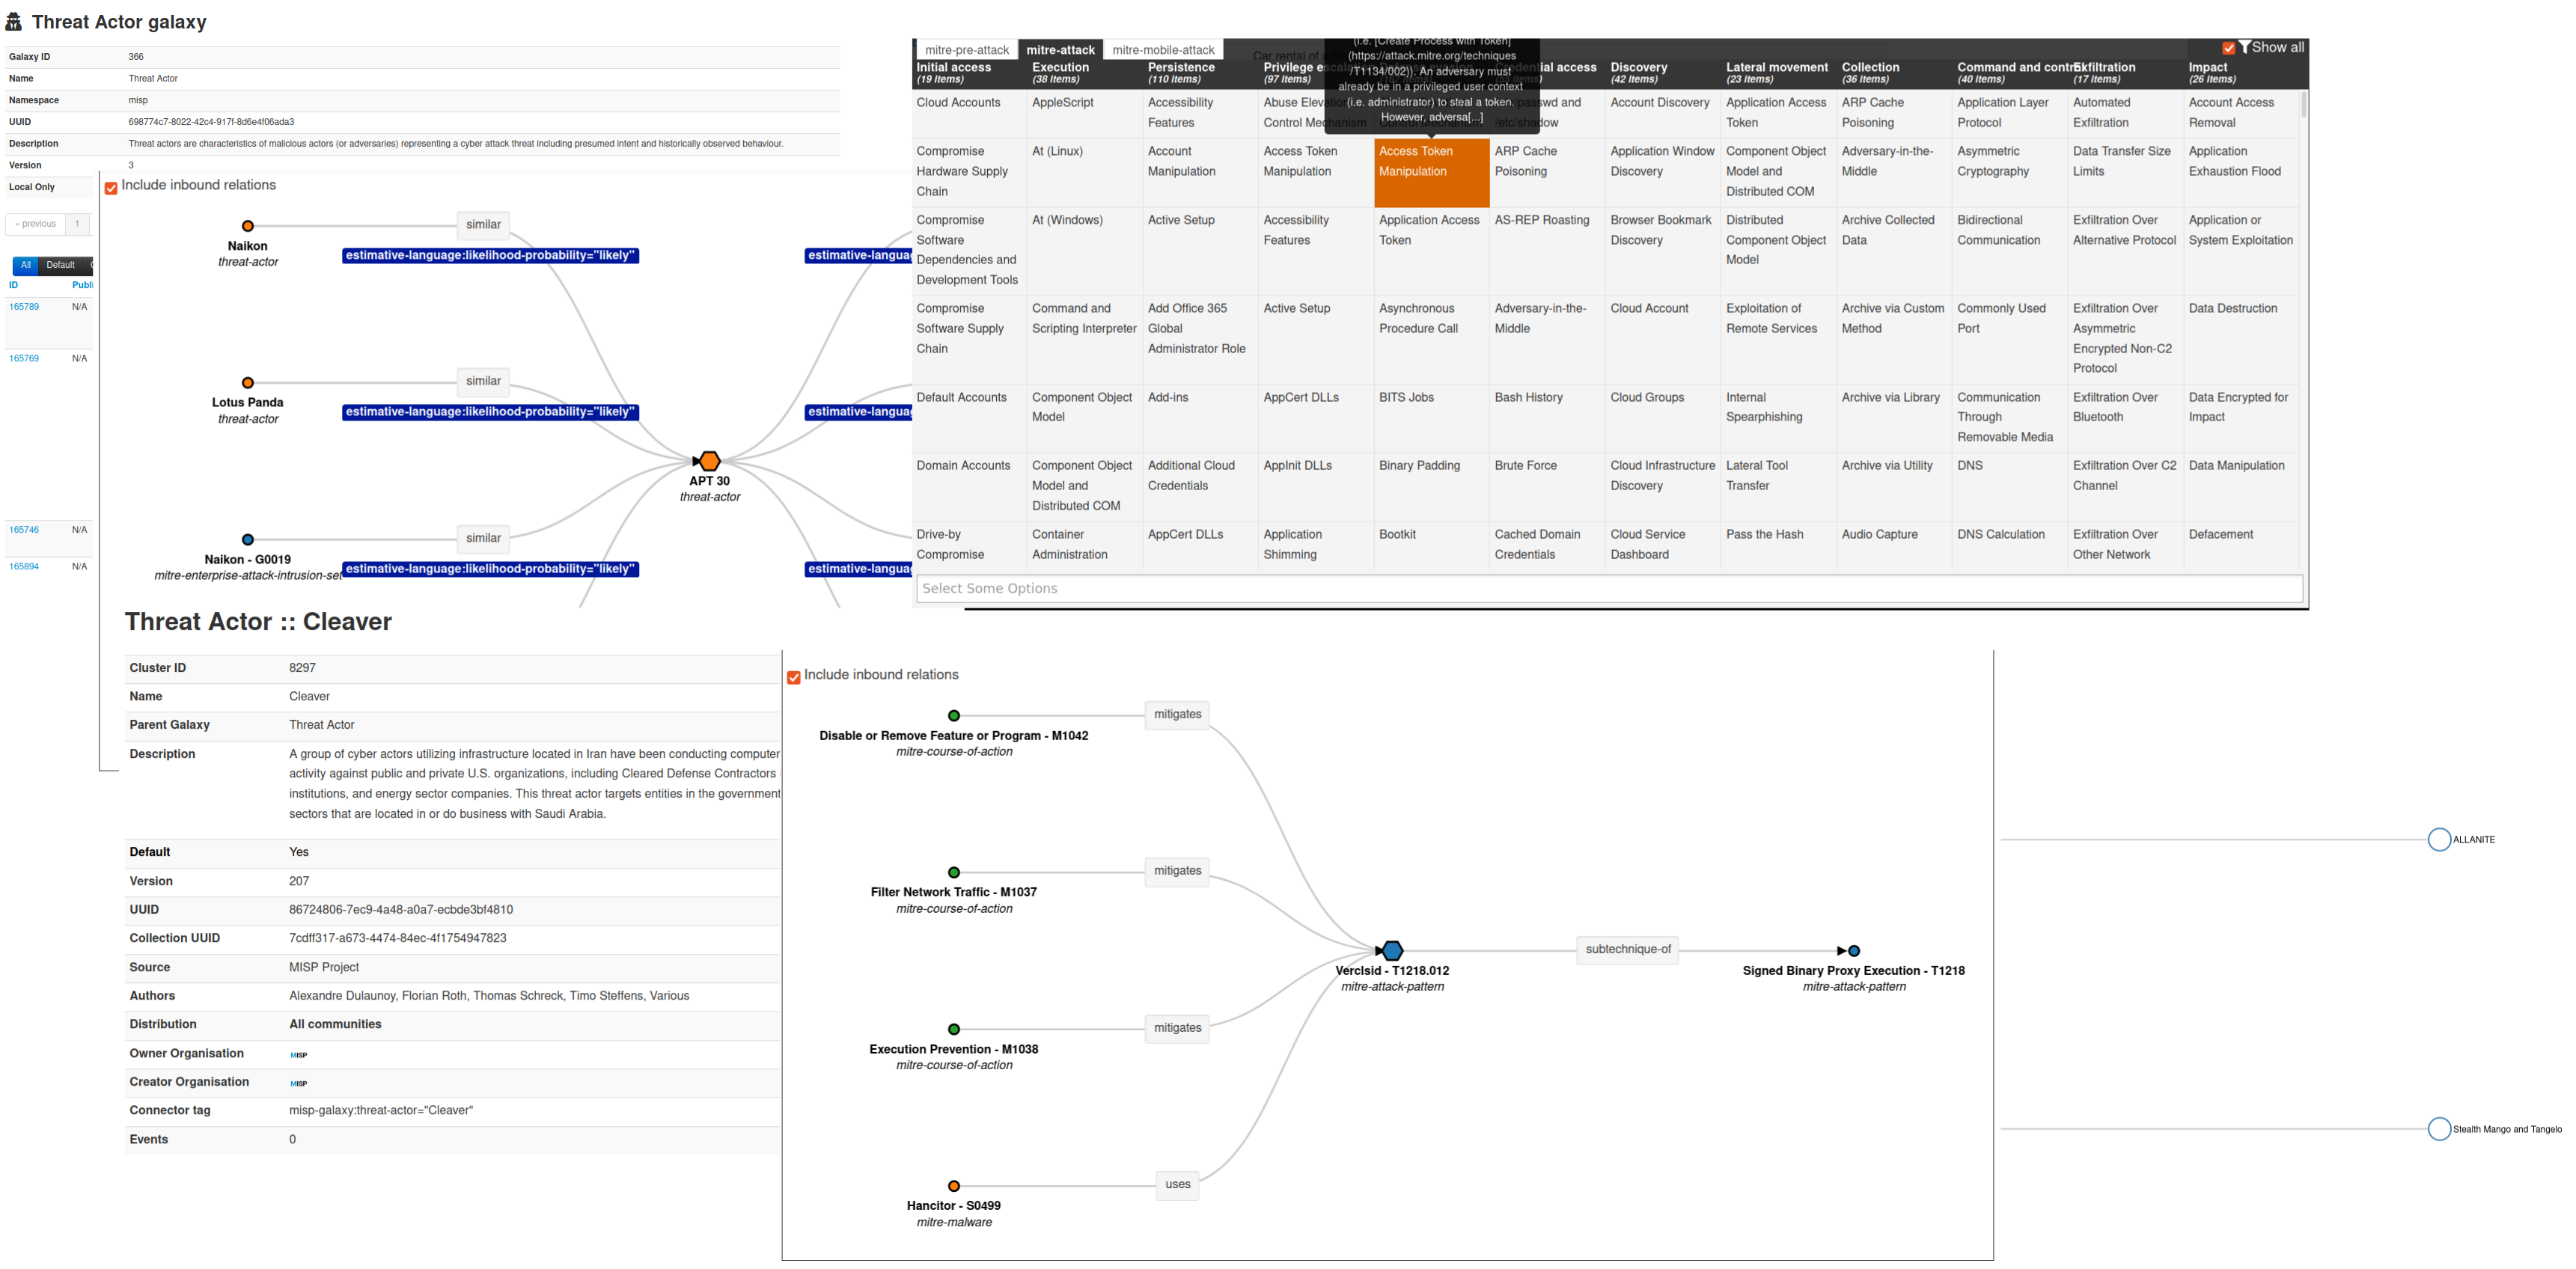
\includegraphics[width=0.84\linewidth]{galaxy_montage.png}
    \end{center}
    \begin{itemize}
        \item Standardized Knowledge Base and Vocabularies to address the Who, What, How and Why
        \item Examples:
        \begin{itemize}
            \item Threat Actors
            \item Countries
            \item Attack Techniques
            \item Campaigns
            \item And \textbf{many more} $\cdots$
        \end{itemize}
    \end{itemize}
\end{frame}

\begin{frame}
    \frametitle{Integration and Automation ecosystem}
    MISP has many features to help you integrate various tools, processes and workflows:
    \begin{itemize}
        \item REST-full \textbf{API} \& \textbf{PyMISP}
        \item \textbf{PubSub / Streaming channels}
        \item \textbf{Enrichment} \& \textbf{Import/Export} service through MISP-modules
        \item \textbf{Workflow system}: Quick and easy automation based on trigger/conditions/actions blocks
    \end{itemize}
\end{frame}

\begin{frame}
    \frametitle{Information Quality Management}
    \begin{center}
        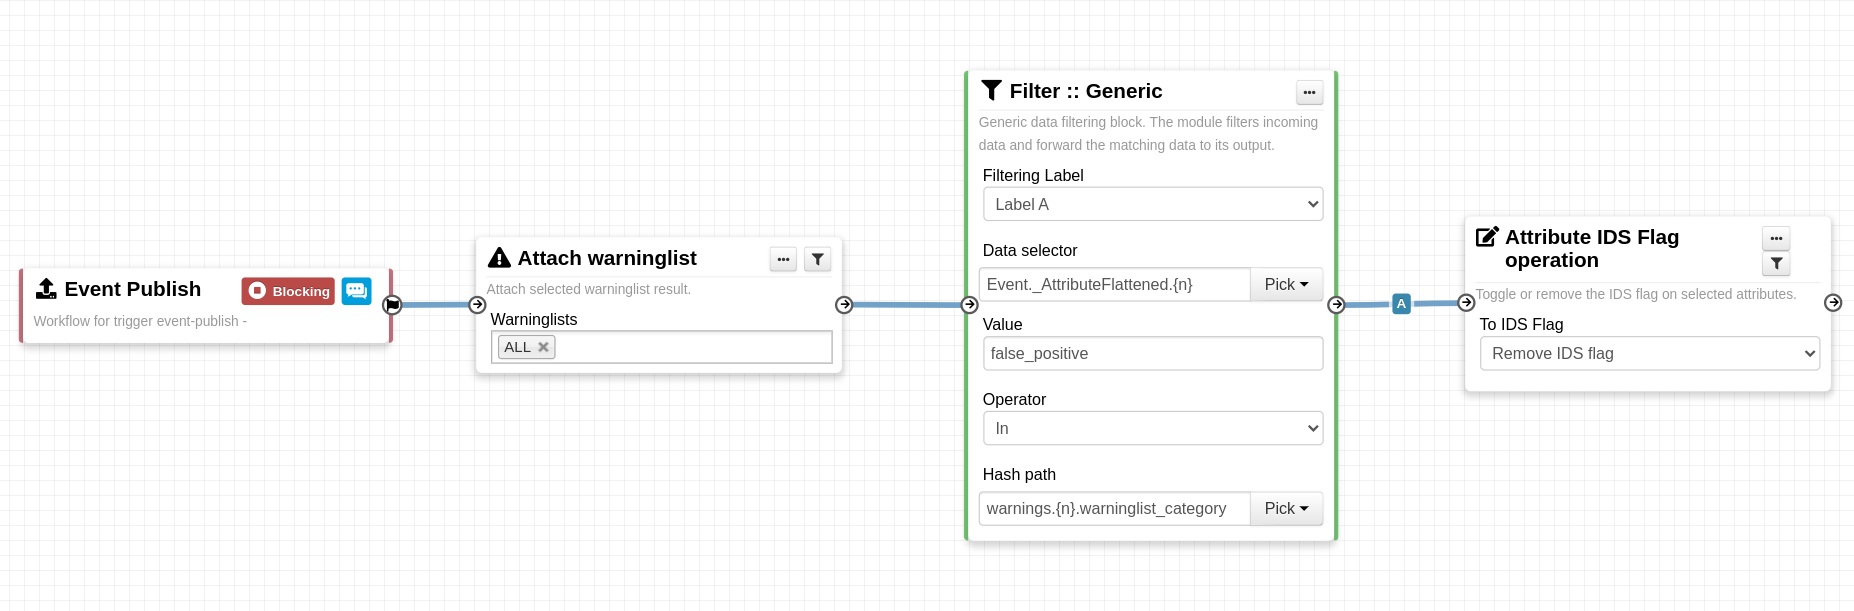
\includegraphics[width=0.99\linewidth]{wf-false-positive.png}
    \end{center}
    \begin{center}
        \textbf{Blueprint library} available on Github\footnote{\url{https://github.com/MISP/misp-workflow-blueprints}}
    \end{center}
\end{frame}

\begin{frame}
    \frametitle{Using the Power of the Community}
    MISP has many features to foster collaboration. To name a few:
    \begin{itemize}
        \item \textbf{Collaboration}: Proposals, Sightings, Extended Events
        \item \textbf{Discussion \& Opinions}: Analyst Data
        \item \textbf{Specialized Sharing}: Delegation, Sharing-Groups
        \item $\cdots$
    \end{itemize}
\end{frame}

\begin{frame}
    \frametitle{Using the Power of the Community}
    \begin{center}
        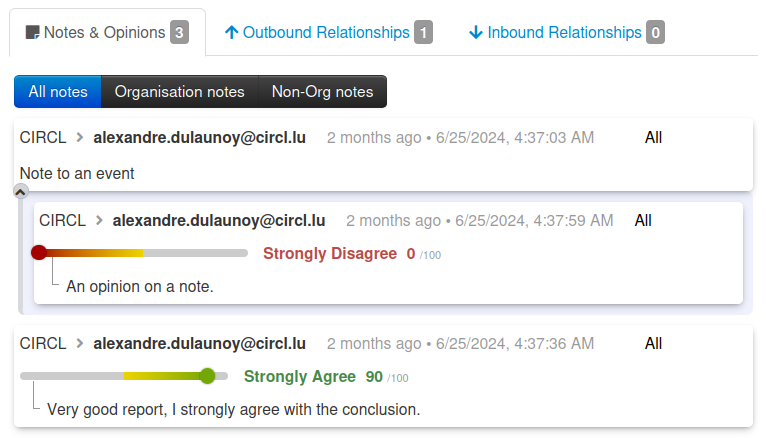
\includegraphics[width=0.85\linewidth]{analyst-data.png}
    \end{center}
\end{frame}

\begin{frame}
    \frametitle{Future of MISP: What's Ongoing}
    \textbf{Long Term:} Major Version \texttt{3.0}
    \begin{itemize}
        \item Focus on the UI.
        \item Revamp front-end and aesthetics.
        \item Analyst-centric perspective.
        \item Graph based data exploration.
        \item Improved search and analytics.
    \end{itemize}
\end{frame}

% \begin{frame}
%     \frametitle{CIRCL's MISP Professional Services (MPS)}
%     \begin{itemize}
%         \item We are comfortably funded to ensure the project's continued prosperity.
%         \item MPS provides professional services and assists organizations seeking to secure support for MISP.
%     \end{itemize}
%     \vspace{1em}
%     \textbf{CIRCL's Offering:}
%     \begin{itemize}
%         \item \textbf{Support Contract:} Prioritized issue resolution and expert guidance.
%         \item \textbf{Training:} Tailored to the expertise level of participants.
%             \begin{itemize}
%                 \item {\small Free onboarding MISP training for ISACs and their members.}
%             \end{itemize}
%         \item \textbf{Hosting:} Hosted on our infrastructure in Luxembourg (LU), available as virtual or dedicated instances.
%             \begin{itemize}
%                 \item {\small OS and MISP maintenance, with early patching for security issues.}
%             \end{itemize}
%     \end{itemize}
% \end{frame}

% \begin{frame}
%     \frametitle{Conclusion}
%     \begin{itemize}
%         \item MISP is just a tool — what truly matters are your \textbf{sharing and analysis practices}.
%         \item MISP strives to meet the use cases of any community, from simple to complex ones.
%         \item The MISP project combines \textbf{open-source software}, \textbf{open standards}, and \textbf{best practices} to make information sharing and analysis a reality.
%     \end{itemize}
% \end{frame}

\section{Sharing Models and Distributions}
\begin{frame}
    \frametitle{MISP Distribution}
    \begin{minipage}[t]{0.6\textwidth}
        \vspace{0pt}
        MISP offers fine-grained distribution mechanism:
        \begin{itemize}
            \item Many {\bf distribution level} offering granularity
            \item Sharing via distribution lists - {\bf Sharing groups}
        \end{itemize}
        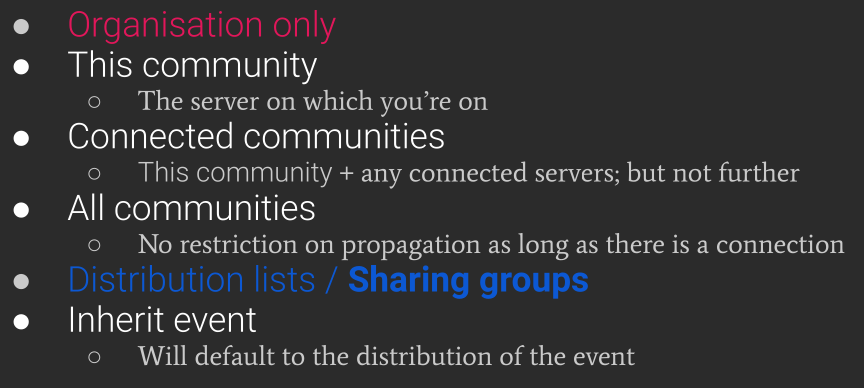
\includegraphics[width=0.9\linewidth]{distribution-list.png}
    \end{minipage}%
    \begin{minipage}[t]{0.4\textwidth}
        \vspace{0pt}
        \centering
        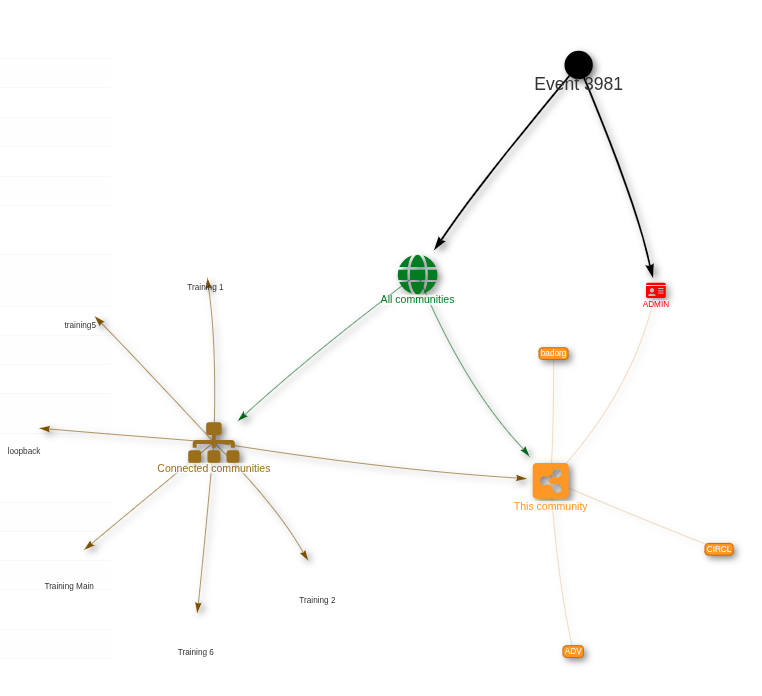
\includegraphics[width=0.95\linewidth]{distribution-graph.png}
    \end{minipage}%
\end{frame}

\begin{frame}
    \frametitle{MISP Sharing}
    \begin{itemize}
        \item User defined {\bf filtered sharing} for all the above mentioned methods
        \item Cross-instance information {\bf caching} for quick lookups of large data-sets
        \item Support for multi-MISP \textbf{internal enclaves}
    \end{itemize}
    \begin{center}
        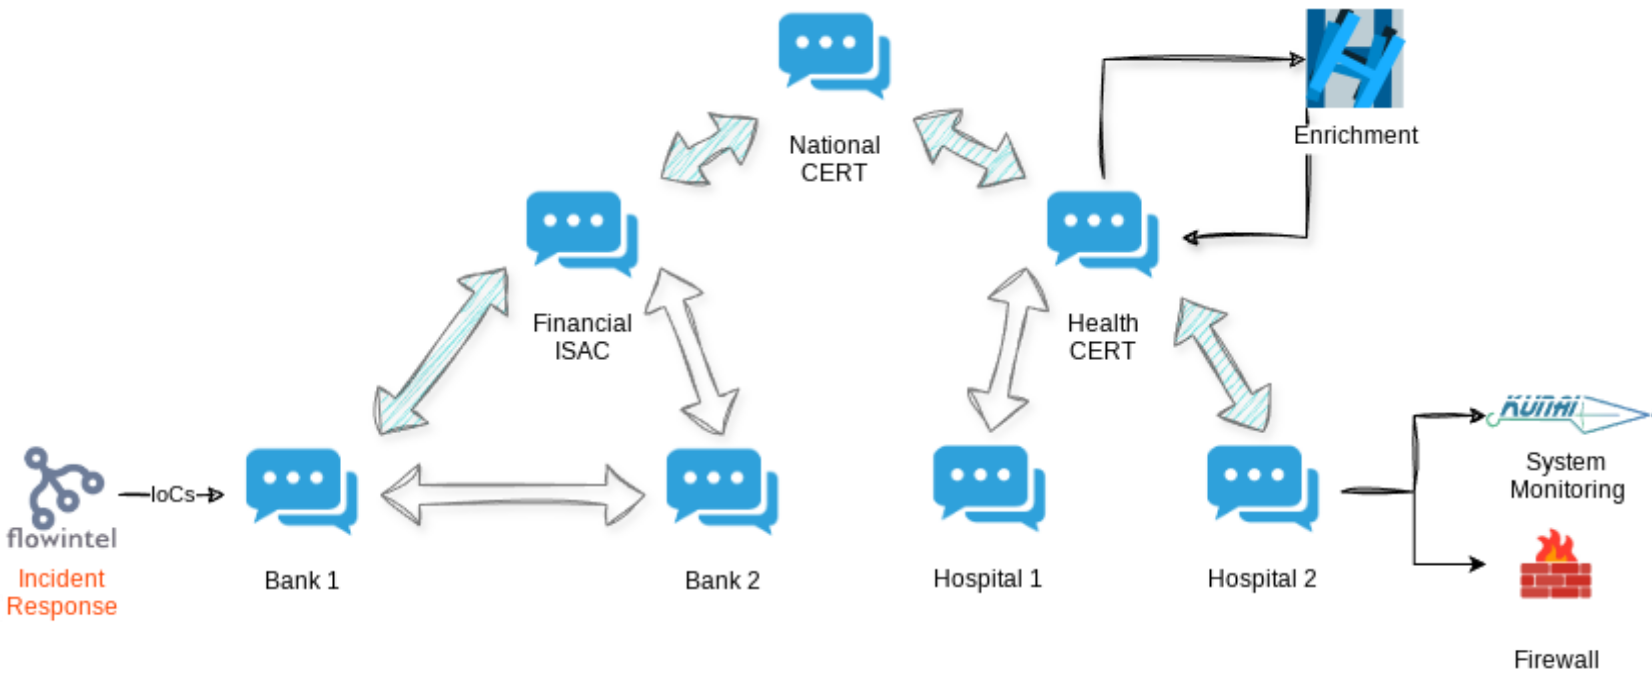
\includegraphics[width=0.80\linewidth]{misp-infosharing.png}
    \end{center}
\end{frame}


\section{Correlation with tradional cybercrime: DDOS on governmental infrastructure}
\begin{frame}
    \frametitle{DDOS on governmental infrastructure}

    \begin{itemize}
        \item Public facing webserver
        \item Hosted by GROUPEMENT D'INTERET PUBLIC GIGALIS
        \item Located in France
        \item Autonomous system number: \texttt{AS47608}
        \item Announced subnet: \texttt{80.82.224.0/20}
        \item Relying on Microsoft 365 / Outlook email security infrastructure
    \end{itemize}
\end{frame}

\begin{frame}
    \frametitle{DDOS on governmental infrastructure}

    \begin{center}
        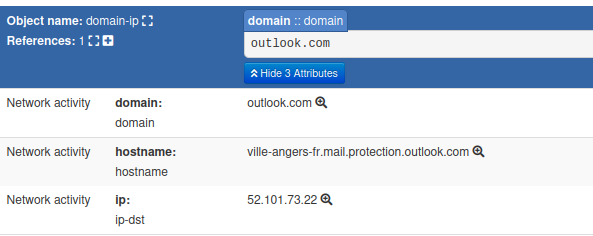
\includegraphics[width=0.6\linewidth]{angers-network.png}
    \end{center}

    \begin{center}
        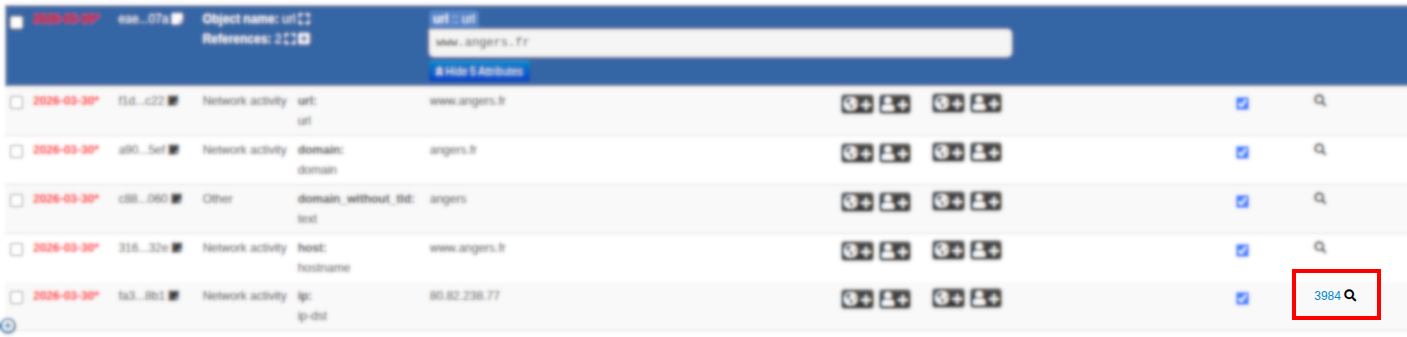
\includegraphics[width=0.95\linewidth]{ddosio-angers.png}
    \end{center}
\end{frame}

\begin{frame}
    \frametitle{DDOS on governmental infrastructure}
     \begin{center}
        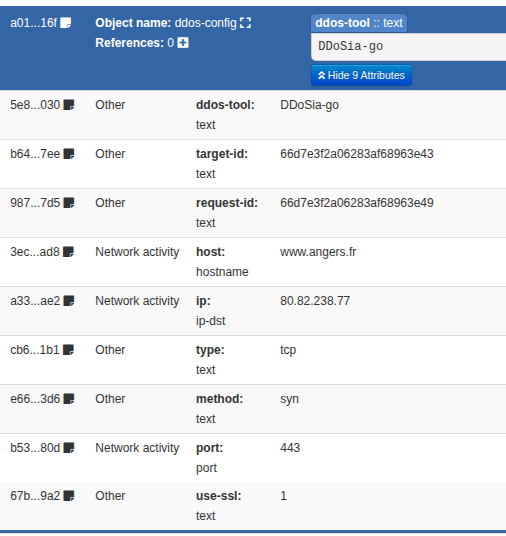
\includegraphics[width=0.6\linewidth]{ddosia-config}
    \end{center}
\end{frame}


\section*{Election Security}
\subsection{Case Study: Article from Direkt36}
\begin{frame}
    \frametitle{Event \& Reports}
    \textbf{Summary}: The event describes a reported covert effort targeting the Tisza Party's internal systems. The central figure in the narrative is an unknown actor using the alias Henry, who allegedly tried to recruit a young IT-linked former volunteer and leverage insider access to monitor, destabilize, or potentially disrupt Tisza infrastructure
     \begin{center}
        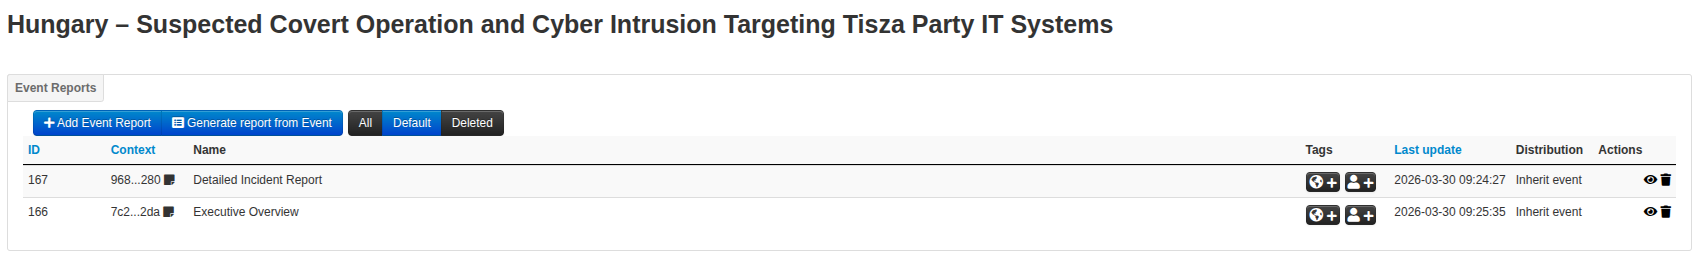
\includegraphics[width=1.0\linewidth]{direkt36_event.png}
    \end{center}
\end{frame}

\begin{frame}
    \frametitle{Event Data}
    \begin{minipage}[t]{0.4\textwidth}
        \vspace{0pt}
        \textbf{Objects of interest}:
        \begin{itemize}
            \item \texttt{Person}
            \item \texttt{Legal Entity}
            \item \texttt{Incident}
            \item \texttt{Leaked Document}
            \item ...
        \end{itemize}
    \end{minipage}%
    \begin{minipage}[t]{0.6\textwidth}
        \vspace{0pt}
        \centering
        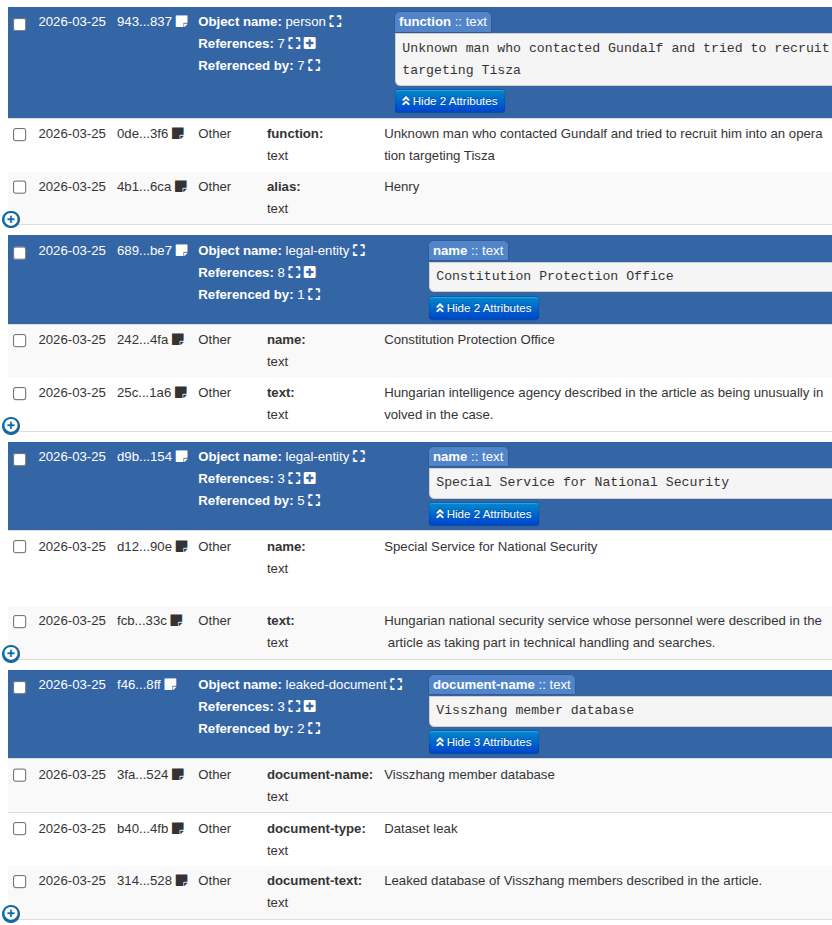
\includegraphics[width=0.99\linewidth]{direkt36_data.png}
    \end{minipage}%
\end{frame}

\begin{frame}
    \frametitle{Event Graph}
     \begin{center}
        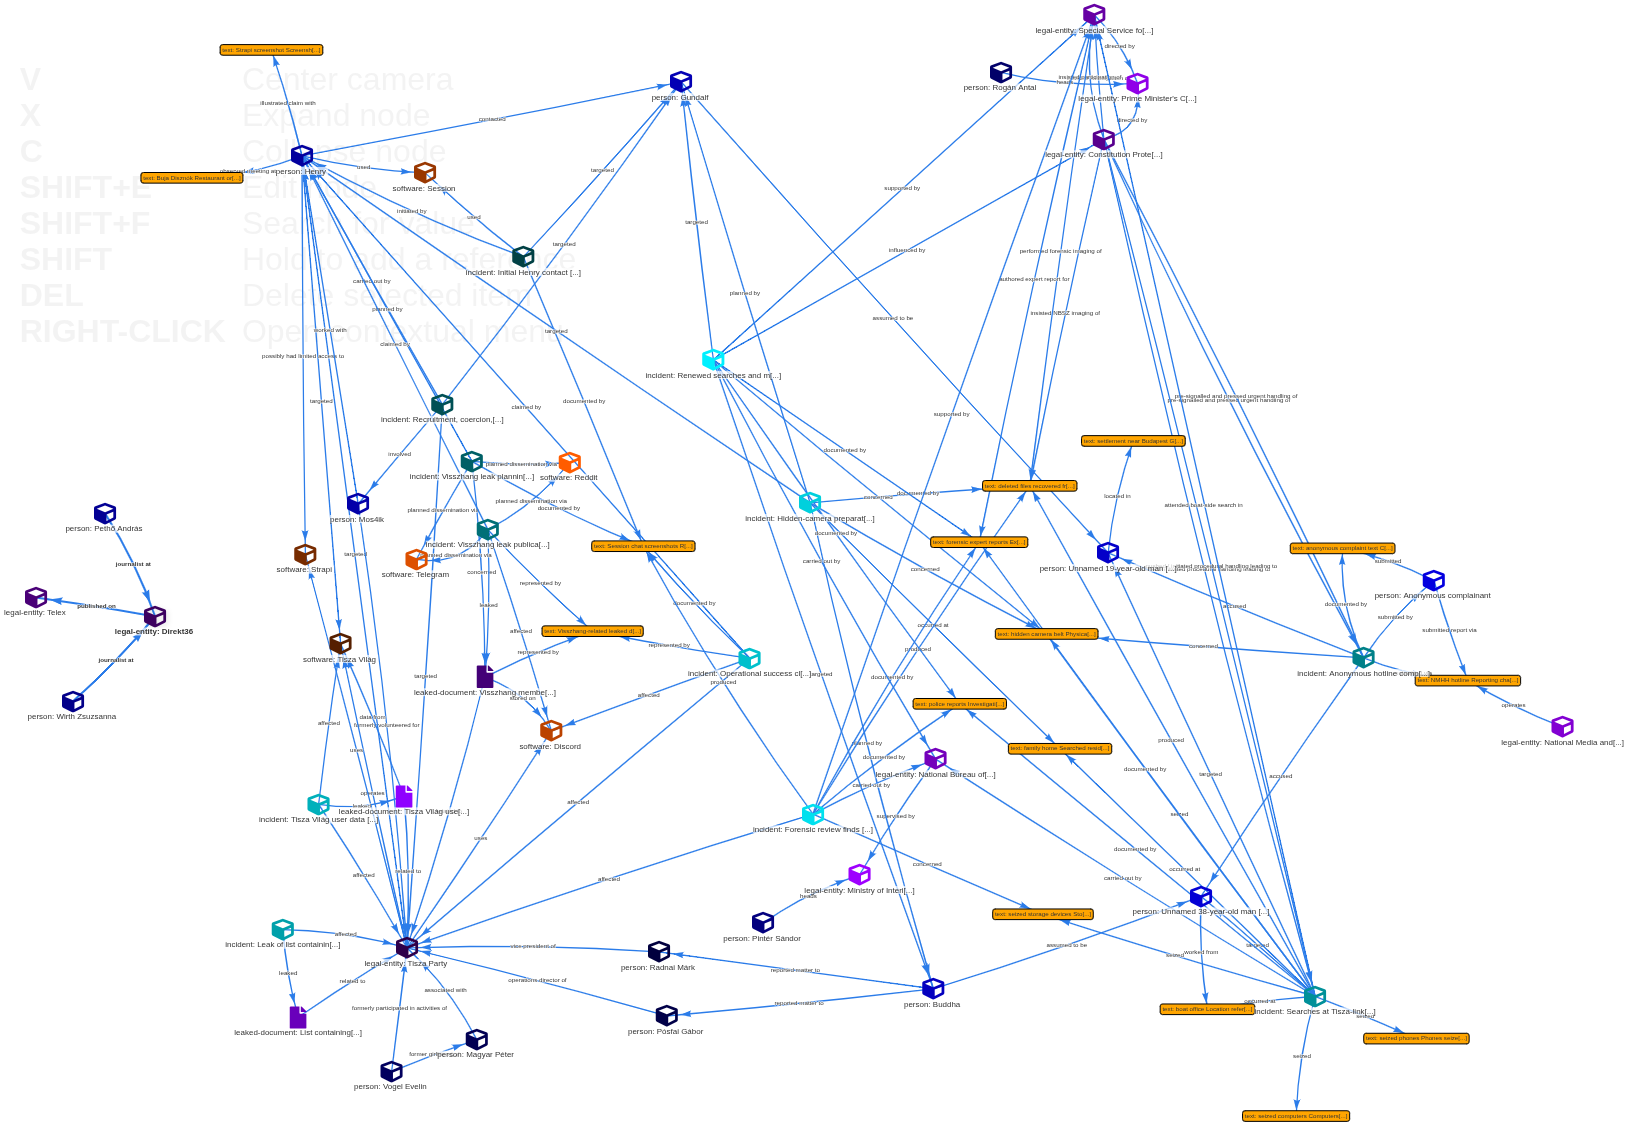
\includegraphics[width=0.95\linewidth]{direkt36_graph.png}
    \end{center}
\end{frame}

\begin{frame}
    \frametitle{Event Timeline}
     \begin{center}
        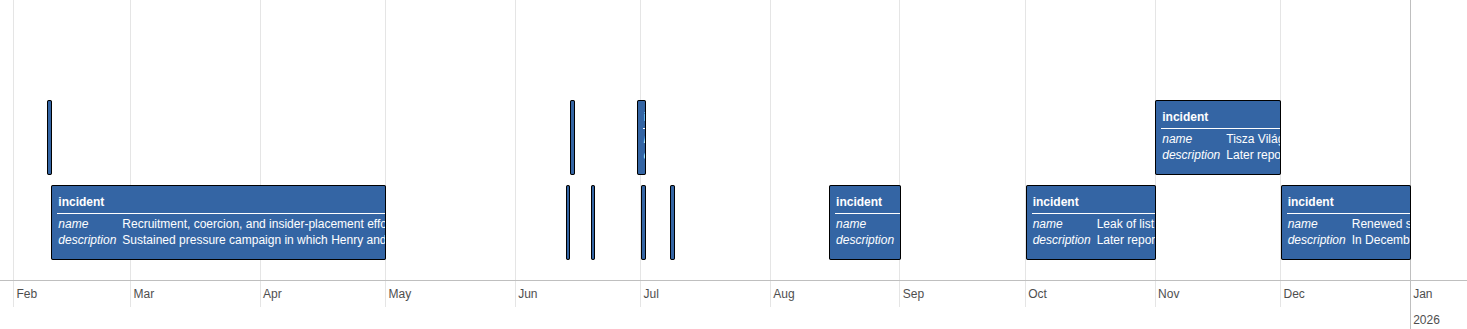
\includegraphics[width=0.95\linewidth]{direkt36_timeline.png}
        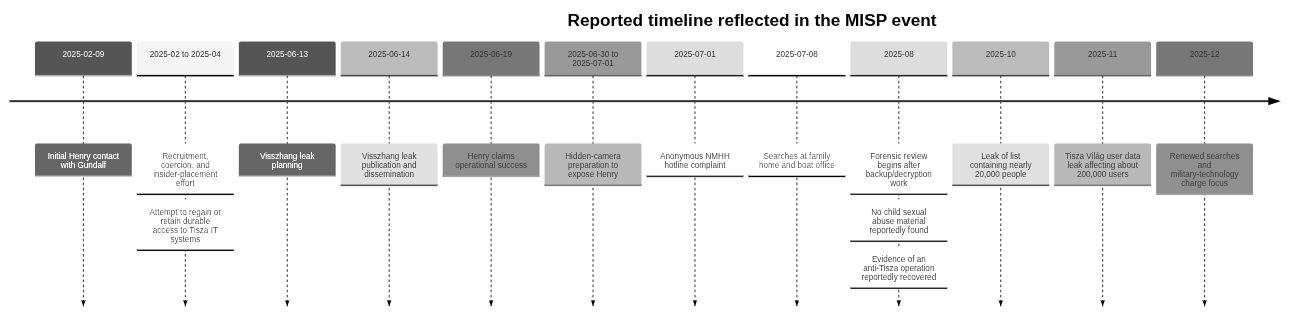
\includegraphics[width=0.95\linewidth]{direkt36_timeline2.png}
    \end{center}
\end{frame}

\begin{frame}
    \frametitle{Misinformation \& Election Guidlines}
     \begin{center}
        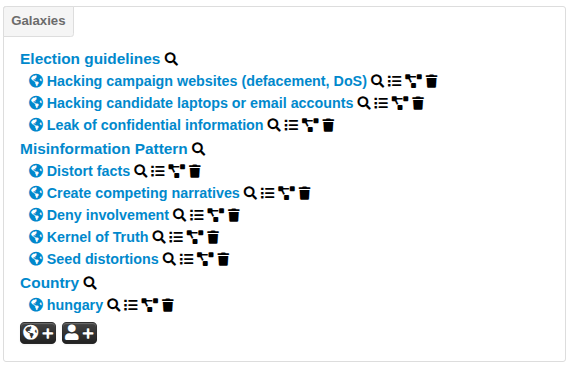
\includegraphics[width=0.95\linewidth]{direkt36_context.png}
    \end{center}
\end{frame}

\subsection{Misinformation \& Election Guidlines Galaxies}
\begin{frame}
    \frametitle{Misinformation \& Election Guidlines Galaxies}
     \begin{center}
        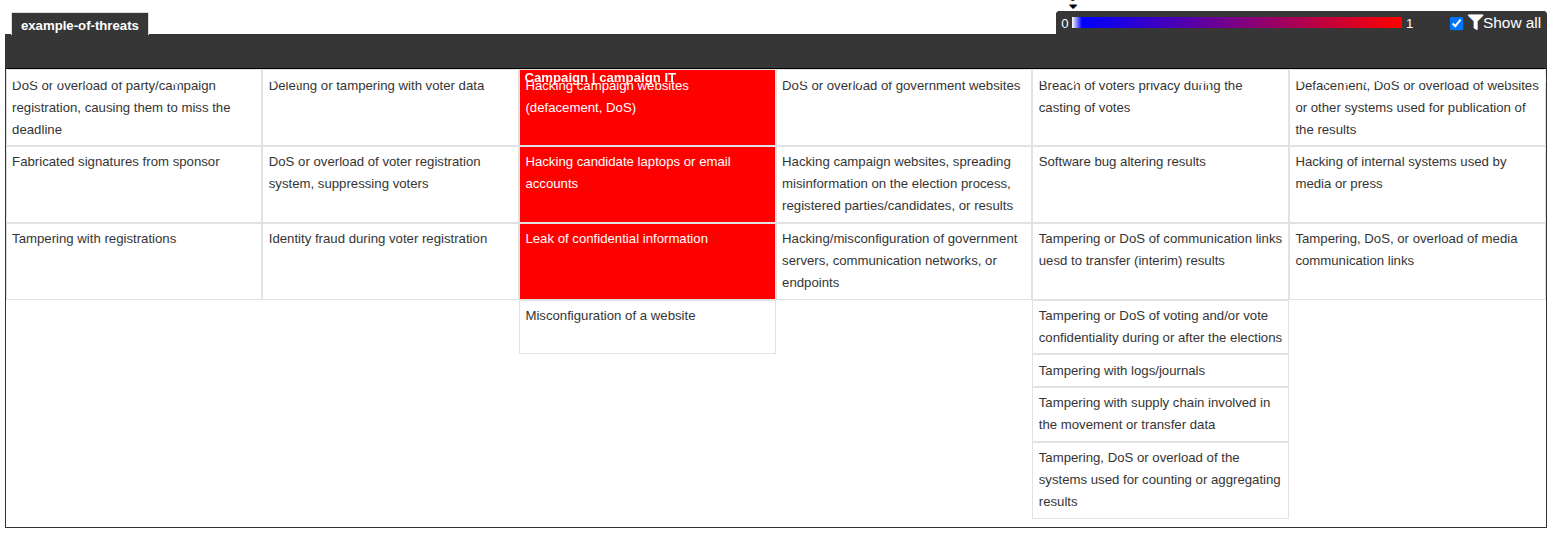
\includegraphics[width=0.95\linewidth]{election-guidelines.png}
    \end{center}
\end{frame}
\begin{frame}
    \frametitle{Misinformation \& Election Guidlines Galaxies}
     \begin{center}
        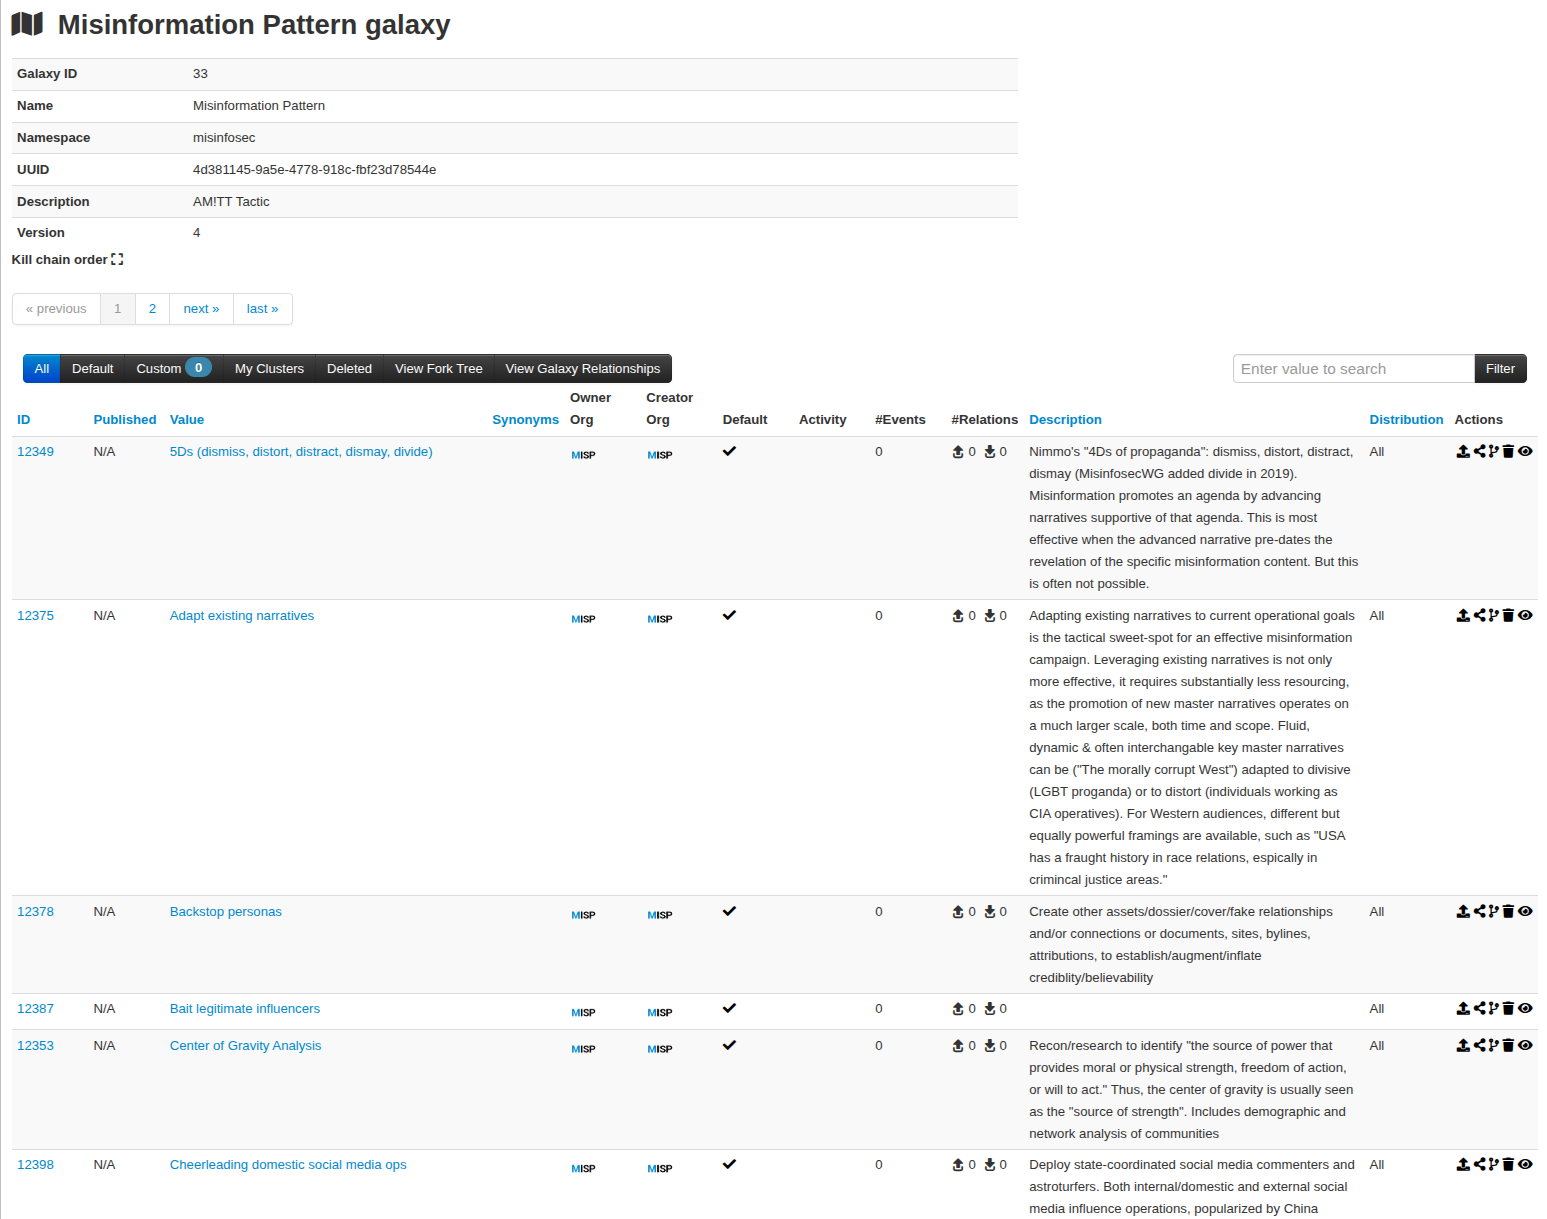
\includegraphics[width=0.95\linewidth]{misinformation_pattern.png}
    \end{center}
\end{frame}


\begin{frame}
     \frametitle{Contact}
     \begin{itemize}
        \item \url{info@circl.lu} - \url{info@misp-project.org}
        \item Open source software developed and used by CIRCL - \url{https://tinyurl.com/ISACTOOLING}
     \end{itemize}
\end{frame}


